\documentclass[12pt]{article}

\usepackage{amsmath, mathtools}
\usepackage{amsfonts}
\usepackage{amssymb}
\usepackage{graphicx}
\usepackage{colortbl}
\usepackage{xr}
\usepackage{hyperref}
\usepackage{longtable}
\usepackage{xfrac}
\usepackage{tabularx}
\usepackage{float}
\usepackage{booktabs}
\usepackage{caption}
\usepackage{pdflscape}
\usepackage{afterpage}

\usepackage[round]{natbib}

\hypersetup{
    bookmarks=true,         % show bookmarks bar?
    colorlinks=true,       % false: boxed links; true: colored links
    linkcolor=red,          % color of internal links (change box color with linkbordercolor)
    citecolor=green,        % color of links to bibliography
    filecolor=magenta,      % color of file links
    urlcolor=cyan           % color of external links
}

%% Comments

\usepackage{color}

\newif\ifcomments\commentstrue %displays comments
%\newif\ifcomments\commentsfalse %so that comments do not display

\ifcomments
\newcommand{\authornote}[3]{\textcolor{#1}{[#3 ---#2]}}
\newcommand{\todo}[1]{\textcolor{red}{[TODO: #1]}}
\else
\newcommand{\authornote}[3]{}
\newcommand{\todo}[1]{}
\fi

\newcommand{\wss}[1]{\authornote{blue}{SS}{#1}} 
\newcommand{\plt}[1]{\authornote{magenta}{TPLT}{#1}} %For explanation of the template
\newcommand{\an}[1]{\authornote{cyan}{Author}{#1}}

%% Common Parts

\newcommand{\progname}{MTOBridge} % PUT YOUR PROGRAM NAME HERE
\newcommand{\authname}{Team 15, Alpha Software Solutions
\\ Badawy, Adham
\\ Yazdinia, Pedram
\\ Jandric, David
\\ Vakili, Farzad
\\ Vezina, Victor
\\ Chiu, Darren} % AUTHOR NAMES                  

\usepackage{hyperref}
    \hypersetup{colorlinks=true, linkcolor=blue, citecolor=blue, filecolor=blue,
                urlcolor=blue, unicode=false}
    \urlstyle{same}


\graphicspath{{images/}}

\title{Software Requirements Specification\\\progname}

\author{\authname}

\date{}

\begin{document}

\maketitle

\newpage
\pagenumbering{roman}

\tableofcontents

\newpage

\begin{table}[hp]
\caption{Revision History} \label{TblRevisionHistory}
\begin{tabularx}{\textwidth}{llX}
\toprule
\textbf{Date} & \textbf{Developer(s)} & \textbf{Change}\\
\midrule
October 4 & David & Add context/partitioning of work\\
\midrule
October 4 & Adham & First Draft of FRs\\
\midrule
October 4 & Darren & Added some Non-functional Requirements\\
\midrule
October 4 & Victor & Project Issues\\
\midrule
October 5 & Victor & Added some Non-functional Requirements\\
\midrule
October 5 & Darren & Refined Non-functional Requirements\\
\midrule
October 5 & Pedram & Added Individual Product Usecase\\
\midrule
October 5 & Adham & Finished FRs\\
\midrule
October 5 & Adham & Added Likely Changes Table\\
\midrule
October 5 & Farzad & Completed parts of project drivers\\
\midrule
October 5 & Adham & Added Prio. and Phase in Plan for FRs and Reflection Skeleton\\
\midrule
October 5 & Adham & Added Behaviour Overview, Refined Requirements, and added Reflection\\
\midrule
October 5 & Darren & Numbered and traced Non-functional Requirements\\
\midrule
October 5 & Farzad & Completed project drivers and reflection\\
\bottomrule
\end{tabularx}
\end{table}

\newpage

\listoftables
\listoffigures

\newpage

\pagenumbering{arabic}

This document describes the requirements for \progname. The template for the Software
Requirements Specification (SRS) is a subset of the Volere
template~\cite{RobertsonAndRobertson2012}. In addition, we have added a few sections not
in the Volere template: Appendix (and its subsections), Phase in Plan, Behavior Overview, Variables.

\begin{table}

\end{table}

\section{Project Drivers}

\subsection{The Purpose of the Project}
For years, Bridge Engineers in Ontario have based their bridge analysis on the Canadian Highway Bridge Design Code (CHBDC)(CSA S6-19) which typically features 
conservatism and adds excessive costs. This project aims to develop an application ’MTOBridge’ that leverages prepared MATLAB engines 
(containing the logic for novel analysis methods) and better visualizes their outputs while enhancing usability. This enables the refined methods of analysis to 
become routine for bridge design and evaluation. Moreover, A unique feature of ’MTOBridge’, which is otherwise unavailable in other bridge design/evaluation software, 
is that a direct comparison can be obtained between the results obtained from the CHBDC approximate/simplified approach and those from the refined analysis. 
This endeavor will facilitate confidence in using refined analysis for bridge evaluation and design.

\subsection{The Stakeholders}

\subsubsection{The Client}
Ontario Ministry of Transport (MTO) is the sponsor of this project and is making the investment to bring this program to fruition in 
partnership with the McMaster University Civil Engineering Department.
\subsubsection{The Customers}
Civil engineering firms in the bridge design industry. They will dictate whether or not they will adopt this new tool depending on whether it has helped them 
save costs for their clients and how easy it was for their engineers to use the tool.
\subsubsection{Other Stakeholders}
\begin{itemize}
  \item Department of Civil Engineering, McMaster
	\begin{itemize}
	  \item{The proposed program will be directly developed in collaboration with The Department of Civil Engineering. }
	\end{itemize}
  \item Department of Computing and Software, McMaster 
	\begin{itemize}
	  \item{The proposed program will be directly developed by Engineers from The Department of Computing and Software.} 
	\end{itemize}
\end{itemize}

\subsubsection{User Characteristics}
The potential users of this product are civil engineers designing and monitoring bridges. Age group is between 22-65 years old and they can be from wide variety of 
gender and ethnic groups. Civil engineers are not expected to be technology geeks but they have a basic understanding of user interfaces and how to learn to interact 
with them over time. The majority of the users work on cite using workstations, however as a result of the technological advancements there might be engineers that work 
from home.
\subsection{Mandated Constraints}
    \hspace{5mm} \textbf{C.1:} The system shall be able to perform the calculations using the prepared MATLAB Engines. \\
    \textbf{Rationale:} Dr.Yang and her team which are one of the main stakeholders are not going to implement their engines in another language again.\\
    \textbf{Fit Criterion:} The system shall be able to call the appropriate functions within the MATLAB engine to perform the commanded analysis.\\

    \textbf{C.2:} The product shall operate using Windows 10. \\
    \textbf{Rationale:} The client and majority of the customers use Windows 10 and do not wish to change to a later version.\\
    \textbf{Fit Criterion:} The product shall be approved as Windows 10 compliant based on our tests on a Windows machine.\\

    \textbf{C.3:} The product shouldn't require MATLAB to be installed on the end user’s machine to run the MATLAB engines. \\
    \textbf{Rationale:} The majority of the customers do not have MATLAB licenses and chances are they don’t want to purchase them..\\
    \textbf{Fit Criterion:} The product shall be able to use the logic written in MATLAB without needing to install MATLAB.\\\\

\subsection{Naming Conventions and Terminology}
\textbf{Abutment:} A substructure composed of stone, concrete, brick or timber supporting the ends of a single span bridge or the extreme end of a multi-span bridge. 
Usually, it also supports the approach embankment.\\
\textbf{Dead load:} The weight of the permanent, immoveable parts of a structure, such as the towers, cables, and roadway of a bridge.\\
\textbf{Girder:} A horizontal main structural member (as in a building or bridge) that supports vertical loads and that consists of a single piece or of more than one piece 
bound together.\\
\textbf{Live load:} Refers to traffic that moves across the bridge as well as normal environmental factors such as changes in temperature, precipitation, and winds.\\
\textbf{Span:} In engineering parlance means the gap between two supports.\\
\textbf{Truck Platoon:} A close-knit convoy of self driving trucks that can travel faster and closer together than by traditional means. Expected to become common 
in the future.\\
\textbf{Headway:} A term for the space between the last axle of one truck in the platoon and the next axle of the subsequent truck. Used to measure spacing between trucks.\\
\textbf{Concerned Section:} A term used to define the point along the bridge for which the user is interested in viewing the loads placed on it by the platoon.\\
\textbf{Critical Section:} A term used to mean the point along the bridge that experiences the highest loads during the platoon's trip along the bridge.\\
\textbf{Discretization Length:} This length determines how many sections the user wants to split their bridge into for the critical section calculation. For example,
a 10m long bridge with a discretization length of 1m would be split into 10 sections 1m apart. These 10 would then be compared over the course of the trip to find the 
critical section.\\  

\subsection{Relevant Facts and Assumptions}
\textbf{A.1:} The prepared MATLAB engines are reliable and thoroughly tested.\\
\textbf{A.2:} Users have access to computers that runs Windows 10 and can handle calculation intensive analysis.

\section{Functional Requirements}
\subsection{Behavioral Overview}
The following few paragraphs comprise a verbal summary of the whole of section 2, for quick reference.\\\\

\noindent The Program to be developed is a graphical user interface between the user and a duo of MATLAB solvers created by the Department of Civil Engineering at McMaster
for load rating bridges as a truck platoon drives over them. It will allow the user to interface with the calculations in four major ways. Namely, these are:\\\\ 

\noindent 1. Determining the specifics of the truck platoon that will be rolling over their bridge, in terms of the configuration of the trucks themselves, the number of trucks in
the platoon, the headway between them, and their travel speed.\\\

\noindent 2. Determining the specifics of the bridge their truck platoon will be rolling over, in terms of whether it is a one or two span bridge, how long it is, and what 
material it is made out of.\\\\

\noindent 3. Determining what they want to know about the demands placed on their bridge by the truck platoon. Namely, do they care about what happens to a particular section 
over the course of the trip? Or do they wish to know wish section experiences the highest load over the course of the whole trip?\\\\

\noindent 4. Visualizing the results of the calculations in a comprehensive and informative fashion.\\\\

\noindent There will be other features to the program as well, such as generating a text based report of the outputs over the course of a session of use, and allowing the user
to save and load their truck and bridge configurations for easy access to oft-used configurations. This is a living document, and more functionality may be added over time,
but for now this about covers it.

\subsection{The Scope of the Work}

\subsubsection{The Context of the Work}

\begin{figure}[H]
  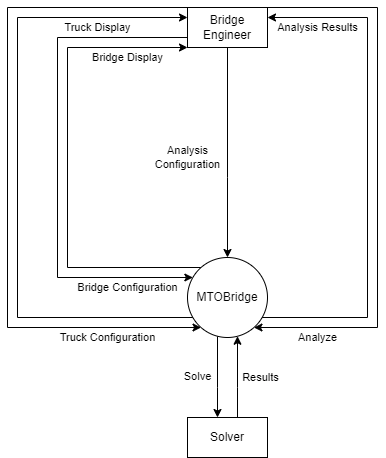
\includegraphics[]{context-diagram.png}
  \caption{Context Diagram of MTOBridge}
  \label {fig:context-diagram}
\end{figure}

\subsubsection{Work Partitioning}

\begin{table}[hp]
  \caption{Business Event List} \label{TblEventList}
  \begin{tabular}{p{0.33\textwidth} | p{0.33\textwidth} | p{0.33\textwidth}}
  \toprule
  \textbf{Event Name} & \textbf{Input/Output} & \textbf{Summary}\\
  \midrule
  Engineer enters truck configuration & IN: Truck configuration, OUT: Truck display & Record truck configuration, show truck visualization\\
  \midrule
  Engineer enters bridge configuration & IN: Bridge configuration, OUT: Bridge display & Record bridge configuration, show bridge visualization\\
  \midrule
  Engineer enters analysis configuration & IN: Analysis configuration & Record analysis configuration\\
  \midrule
  Engineer requests analysis & IN: Analyze request, OUT: Analysis results & Display analysis results\\
  \midrule
  Time to solve forces & OUT: Solve request, IN: Solver results & Give configurations to solver to get results\\
  \bottomrule
\end{tabular}
\end{table}

\subsection{The Scope of the Product}

\subsubsection{Product Boundary}

\begin{figure}[H]
  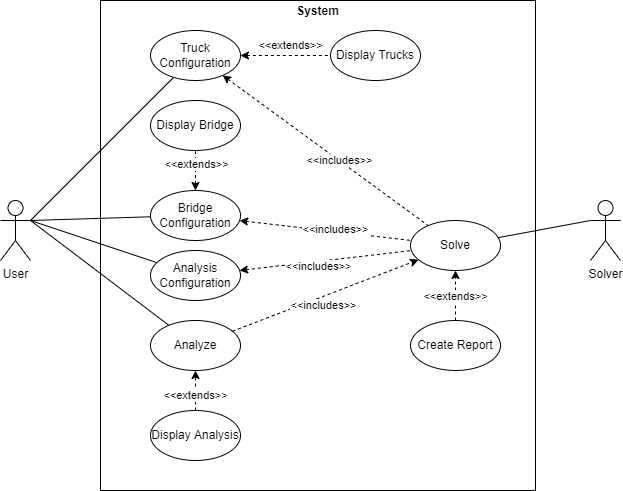
\includegraphics[width=\linewidth]{use-case-diagram.png}
  \caption{Use Case Diagram of MTOBridge}
  \label {fig:use-case-diagram}
\end{figure}

\subsubsection{Variables}
\begin{table}[H]
  \caption{Variable List} \label{TblVariableList}
  \begin{tabular}{p{0.3\textwidth} | p{0.2\textwidth} | p{0.5\textwidth}}
  \toprule
  \textbf{Name} & \textbf{Type} & \textbf{Description}\\
  \midrule
  analyze & bool & User has requested analysis?\\
  \midrule
  displayTrucks & bool & Display truck visualization?\\
  \midrule
  displayBridge & bool & Display bridge visualization?\\
  \midrule
  displayResults & bool & Display analysis results?\\
  \midrule\
  okPressed & bool & Represents whether or not invalid message was accepted\\
  \midrule
  validateTruck & bool & Is validation done on truck configuration?\\
  \midrule
  validateBridge & bool & Is validation done on bridge configuration?\\
  \midrule
  validateAnalysisConfig & bool & Is validation done on analysis configuration?\\
  \midrule
  writeReport & bool & Write results to a file?\\
  \midrule
  input & string & Text representing user input\\
  \midrule
  config & Config & Abstract representation of configuration, with definable fields and options\\
  \midrule
  analysisConfig & Config & Configuration of analysis\\
  \midrule
  bridgeConfig & Config & Configuration of a bridge\\
  \midrule
  truckConfig & Config & Configuration of truck platoon, contains many fields\\
  \midrule
  results & SolverResults & Abstract representation of output from Solver\\
  \bottomrule
\end{tabular}
\end{table}

\subsubsection{Individual Product Use Cases}

\noindent
\textbf{User navigates to the Truck Configuration Tab} \\
\textbf{  Primary Actors:} Engineers\\
\textbf{  Pre Condition:} None\\
\textbf{  Post Condition:} Input values from the user conforms to the valid range required for the calculations.\\ 
\textbf{  Basic Flow:} 
\begin{itemize}
\item System asks user to enter a truck parameter.
\item User enters truck parameter.
\item System checks parameter.
\subitem \textbf{Alternative} If the parameter is incorrect, the user is alerted.
\end{itemize}
\textbf{  Extension:}
\begin{itemize}
\item User requests an animation of the truck platoon.
\item System provides an animation of the truck platoon.
\item User interacts with the animation of the trucks. 
\end{itemize}
\begin{figure}[H]
  \centering
  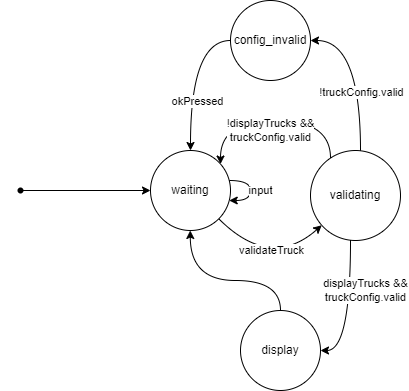
\includegraphics[width=0.5\linewidth]{use-case-1-sm.png}
  \caption{Use Case 1 State Machine}
  \label {fig:use-case-1-sm}
\end{figure}

\noindent
\textbf{User navigates to the Bridge Configuration Tab} \\
\textbf{  Primary Actors:} Engineers\\
\textbf{  Pre Condition:} None\\
\textbf{  Post Condition:} Input values from the user conforms to the valid range required for the calculations.\\ 
\textbf{  Basic Flow:} 
\begin{itemize}
\item System asks the user to enter a bridge parameter. 
\item User enters the bridge parameters. 
\item System checks parameter.
\subitem \textbf{Alternative} If the parameter is incorrect, the user is alerted.
\end{itemize}
\textbf{  Extension:}
\begin{itemize}
\item User requests an animation of the bridge. 
\item System provides an animation of the bridge.
\item User interacts with the animation of the bridge.
\end{itemize}
\begin{figure}[H]
  \centering
  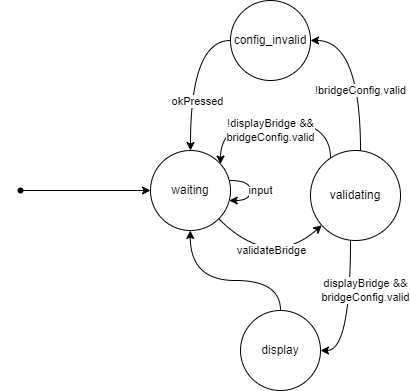
\includegraphics[width=0.5\linewidth]{use-case-2-sm.png}
  \caption{Use Case 2 State Machine}
  \label {fig:use-case-2-sm}
\end{figure}

\noindent
\textbf{User navigates to the Analysis Configuration Tab} \\
\textbf{  Primary Actors:} Engineers\\
\textbf{  Pre Condition:} None\\
\textbf{  Post Condition:} Input values from the user conforms to the valid range required for the calculations.\\ 
\textbf{  Basic Flow:} 
\begin{itemize}
\item System asks the user to enter an analysis parameter. 
\item User enters the analysis parameters. 
\item System checks parameter.
\subitem \textbf{Alternative} If the parameter is incorrect, the user is alerted.
\end{itemize}
\begin{figure}[H]
  \centering
  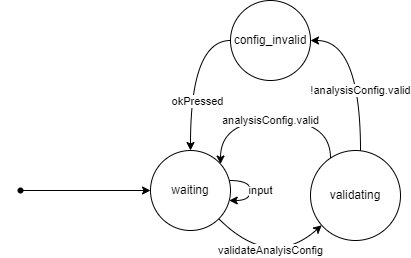
\includegraphics[width=0.5\linewidth]{use-case-3-sm.png}
  \caption{Use Case 3 State Machine}
  \label {fig:use-case-3-sm}
\end{figure}

\noindent
\textbf{User starts the Analyze process. } \\
\textbf{  Primary Actors:} Engineers\\
\textbf{  Pre Condition:} None\\
\textbf{  Post Condition:} None\\ 
\textbf{  Basic Flow:} 
\begin{itemize}
\item User selects the Analyze tab. 
\item The system validates the configurations.
\subitem \textbf{Alternative} If the configurations are not correct, the user is alerted.
\item Configurations are sent to Solver. 
\item Text-based result from Solver is returned.
\end{itemize}
\textbf{  Extension:} 
\begin{itemize}
\item Visualization of results is displayed.
\end{itemize}
\begin{figure}[H]
  \centering
  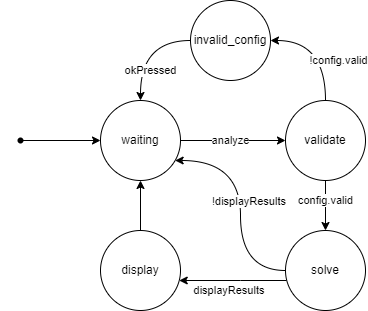
\includegraphics[width=0.5\linewidth]{use-case-4-sm.png}
  \caption{Use Case 4 State Machine}
  \label {fig:use-case-4-sm}
\end{figure}

\noindent
\textbf{The solver solves the mathematical model using the given inputs from the system.} \\
\textbf{  Primary Actors:} Solver\\
\textbf{  Pre Condition:} Truck, Bridge and Analysis Configuration are all valid.\\
\textbf{  Post Condition:} Received results valid based on the testing spec.\\ 
\textbf{  Basic Flow:} 
\begin{itemize}
\item The system receives the configuration data. 
\item The system sends the data to the Solver where the equations are solved using the given parameters. 
\item Solver returns text-based results. 
\subitem \textbf{Alternative} The solver cannot solve the equations using the given input. The user is alerted to check their parameters. 
\end{itemize}
\begin{figure}[H]
  \centering
  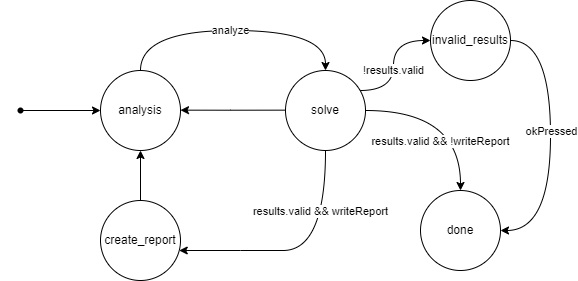
\includegraphics[width=0.5\linewidth]{use-case-5-sm.png}
  \caption{Use Case 5 State Machine}
  \label {fig:use-case-5-sm}
\end{figure}

\subsection{Functional Requirements/Phase in Plan}
  \textbf{FR.1} The Program should be able to call the backend MATLAB functions. \\
  \textbf{Rationale:} To visually display the outputs corresponding to user input, the UI needs to first figure out what those outputs are via the backend MATLAB.\\
  \textbf{Fit Criterion:} Testing will be performed to confirm whether or not the program can successfully call the MATLAB functions.\\
  \textbf{Priority/Phase in Date:} High/Nov 7th\\
  \textbf{Phase in Date Rationale:} This will be the first functionality implemented as it is necessary for proof of concept.\\
  \textbf{Traceability:} C.1, A.1.\\\\
  
  \noindent\textbf{FR.2} The Program should allow the user to define the characteristics of the truck platoon, including truck configuration, number of trucks, headway, and travel speed.\\
  \textbf{Rationale:} The goal of the program is to determine the forces exerted by a given platoon on a bridge, they can come in many different forms, so flexibility in the characteristics
  of the platoon are necessary for the relevance of the simulation.\\ 
  \textbf{Fit Criterion:} At least one method of input(text based, dropdown list, etc) exists that allows users to correctly specify those 4 characteristics of the platoon.\\
  \textbf{Priority/Phase in Date:} Medium/Dec 20th\\
  \textbf{Phase in Date Rationale:} This will be among the later functionalities as while it is very important for the finished product, it is not proof of concept level.\\
  \textbf{Traceability:} N/A: No constraints or assumptions trace to this requirement.\\\\

  \noindent\textbf{FR.3} The Program should allow the user to visualize the effects of their truck platoon characteristic definitions on the final platoon.\\
  \textbf{Rationale:} This is mainly to help the user verify that the inputs they put into the program correspond to the platoon they had in mind. As we are making a GUI,
  visual feedback is paramount to functionality.\\
  \textbf{Fit Criterion:} There exists some visual representation of the truck platoon that changes to correctly reflect the impact of changes in user input.\\
  \textbf{Priority/Phase in Date:} Medium/Jan 5th\\
  \textbf{Phase in Date Rationale:} This will be among the last functionalities implemented as it is dependent on FR.2.\\
  \textbf{Traceability:} N/A: No constraints or assumptions trace to this requirement.\\\\

  \noindent\textbf{FR.4} The Program should allow the user to save their current truck platoon configuration for later use.\\
  \textbf{Rationale:} Users may be interested in testing the demands a particular truck platoon places on bridges disproportionately more often than others,
   in multiple situations, and over multiple sessions. Making it so they don't have to manually remake it every time is important for the efficient use of The Program.\\
  \textbf{Fit Criterion:} The Program is capable of storing a truck platoon configuration in some form to be retrieved later.\\
  \textbf{Priority/Phase in Date:} Low/Jan 25th\\
  \textbf{Phase in Date Rationale:} This will be among the last functionalities implemented as it is among the lowest priority requirements.\\
  \textbf{Traceability:} N/A: No constraints or assumptions trace to this requirement.\\\\

  \noindent\textbf{FR.5} The Program should allow the user to load in their previously saved truck platoon configurations.\\
  \textbf{Rationale:} A companion piece to FR.4, the ability to save a configuration is functionally useless if you can't pull it back out later.\\
  \textbf{Fit Criterion:} The Program is capable of correctly recreating a truck platoon configuration from previously saved data.\\
  \textbf{Priority/Phase in Date:} Low/Jan 30th\\
  \textbf{Phase in Date Rationale:} This will be among the last functionalities implemented as it is among the lowest priority requirements.\\
  \textbf{Traceability:} N/A: No constraints or assumptions trace to this requirement.\\\\

  \noindent\textbf{FR.6} The Program should allow the user to define the characteristics of the bridge, including what type of bridge it is, its length, and what material it
  is made of.\\
  \textbf{Rationale:} Different bridges will react to the same truck platoon differently, therefore specifying the relevant characteristics of the bridge is necessary for
  the relevance of the simulation.\\
  \textbf{Fit Criterion} At least one method of input(text based, dropdown list, etc) exists that allows users to correctly specify those 3 characteristics of the bridge.\\
  \textbf{Priority/Phase in Date:} Medium/Dec 20th\\
  \textbf{Phase in Date Rationale:} This will be among the later functionalities as while it is very important for the finished product, it is not proof of concept level.\\
  \textbf{Traceability:} N/A: No constraints or assumptions trace to this requirement.\\\\
  
  \noindent\textbf{FR.7} The Program should allow the user to visualize the effects of their bridge characteristic definitions on the final bridge.\\
  \textbf{Rationale:} This is mainly to help the user verify that the inputs they put into the program correspond to the bridge they had in mind. As we are making a GUI,
  visual feedback is paramount to functionality.\\
  \textbf{Fit Criterion:} There exists some visual representation of the bridge that changes to correctly reflect the impact of changes in user input.\\
  \textbf{Priority/Phase in Date:} Medium/Jan 5th\\
  \textbf{Phase in Date Rationale:} This will be among the last functionalities implemented as it is dependent on FR.6.\\
  \textbf{Traceability:} N/A: No constraints or assumptions trace to this requirement.\\\\
  
  \noindent\textbf{FR.8} The Program should allow the user to save their current bridge configuration for later use.\\
  \textbf{Rationale:} Users may be interested in testing a particular bridge configuration disproportionately more often than others, in multiple situations
   and over multiple sessions. Making it so they don't have to manually remake it every time is important for the efficient use of The Program.\\
  \textbf{Fit Criterion:} The Program is capable of storing a bridge configuration in some form to be retrieved later.\\
  \textbf{Priority/Phase in Date:} Low/Jan 25th\\
  \textbf{Phase in Date Rationale:} This will be among the last functionalities implemented as it is among the lowest priority requirements.\\
  \textbf{Traceability:} N/A: No constraints or assumptions trace to this requirement.\\\\

  \noindent\textbf{FR.9} The Program should allow the user to load in their previously saved bridge configurations.\\
  \textbf{Rationale:} A companion piece to FR.8, the ability to save a configuration is functionally useless if you can't pull it back out later.\\
  \textbf{Fit Criterion:} The Program is capable of correctly recreating a bridge configuration from previously saved data.\\
  \textbf{Priority/Phase in Date:} Low/Jan 30th\\
  \textbf{Phase in Date Rationale:} This will be among the last functionalities implemented as it is among the lowest priority requirements.\\
  \textbf{Traceability:} N/A: No constraints or assumptions trace to this requirement.\\\\

  \noindent\textbf{FR.10} The Program should allow the user to define which of the two solvers they are interested in using.\\
  \textbf{Rationale:} As the MATLAB backend can solve for both the demand on a concerned section as the platoon drives along, as well as for which section has the 
  highest maximum demand over the course of the whole trip, and these are very different pieces of info, allowing the user to determine which they are currently interested in 
  is important.\\
  \textbf{Fit Criterion:} At least one method of input(text based, dropdown list, etc) exists that allows the user to accurately choose which solver they are would like to use.\\
  \textbf{Priority/Phase in Date:} High/Nov 20th\\
  \textbf{Phase in Date Rationale:} This functionality will be implemented relatively early as it is an important part of the core program.\\
  \textbf{Traceability:} N/A: No constraints or assumptions trace to this requirement.\\\\

  \noindent\textbf{FR.11} The Program should allow the user to define a section of concern on the bridge.\\
  \textbf{Rationale:} The first solver revolves around calculating the demand on a certain point along the bridge as the truck platoon drives over, specifying what point it is
  that we care about is necessary for this function.\\
  \textbf{Fit Criterion:} At least one method of input(text based, dropdown list, etc) exists that allows the user to accurately determine a section of concern on the bridge.\\
  \textbf{Priority/Phase in Date:} High/Nov 25th\\
  \textbf{Phase in Date Rationale:} This functionality will be implemented relatively early as it is an important part of the core program.\\
  \textbf{Traceability:} N/A: No constraints or assumptions trace to this requirement.\\\\

  \noindent\textbf{FR.12} The Program should allow the user to define a discretization length for their bridge.\\
  \textbf{Rationale:} The second solver finds which section has the maximum demand placed on it over the course of the platoon's trip. The discretization length determines how
  many sections the bridge is split up into, which is necessary for the functioning of the second solver.\\
  \textbf{Fit Criterion:} At least one method of input(text based, dropdown list, etc) exists that allows the user to accurately define a discretization length for their bridge.\\
  \textbf{Priority/Phase in Date:} High/Nov 30th\\
  \textbf{Phase in Date Rationale:} This functionality will be implemented relatively early as it is an important part of the core program.\\
  \textbf{Traceability:} N/A: No constraints or assumptions trace to this requirement.\\\\

  \noindent\textbf{FR.13} The Program should allow the user to define which type of demand placed on the bridge they are interested in, between shear forces and positive/negative moment.\\
  \textbf{Rationale:} There are a variety of different demands placed on the bridge as the platoon drives over, and the MATLAB backend contains calculations for all 3 of the
  above mentioned demands. Allowing the user to define which of the 3 they are interested in seeing is necessary for the functionality of the simulation.\\
  \textbf{Fit Criterion:} At least one method of input(text based, dropdown list, etc) exists that allows the user to correctly define which of the 3 demands they are interested in
  simulating.\\
  \textbf{Priority/Phase in Date:} Medium/Dec 15th\\
  \textbf{Phase in Date Rationale:} This functionality will be implemented somewhere in the middle as it is and important part of the program.\\
  \textbf{Traceability:} N/A: No constraints or assumptions trace to this requirement.\\\\

  \noindent\textbf{FR.14} The Program should be capable of visualizing the results of the concerned section calculation for the user.\\
  \textbf{Rationale:} This is essentially the main purpose of the GUI; displaying the results of the MATLAB backend calculations visually to the user. This is one of the two
  main calculations to be represented, so this functionality is very necessary.\\
  \textbf{Fit Criterion:} There exists an accurate visualization of the mathematical results of the concerned section calculation.\\
  \textbf{Priority/Phase in Date:} Extremely High/Dec 10th\\
  \textbf{Phase in Date Rationale:} While this functionality is THE core feature of the program, its proper implementation depends on many other FRs, so it will be fully implemented on the later side.\\
  \textbf{Traceability:} N/A: No constraints or assumptions trace to this requirement.\\\\

  \noindent\textbf{FR.15} The Program should be capable of visualizing the results of the critical section calculation for the user.\\
  \textbf{Rationale:} This is essentially the main purpose of the GUI; displaying the results of the MATLAB backend calculations visually to the user. This is one of the two
  main calculations to be represented, so this functionality is very necessary.\\
  \textbf{Fit Criterion:} There exists an accurate visualization of the mathematical results of the critical section calculation.\\
  \textbf{Priority/Phase in Date:} Extremely/Dec 10th\\
  \textbf{Phase in Date Rationale:} While this functionality is THE core feature of the program, its proper implementation depends on many other FRs, so it will be fully implemented on the later side.\\
  \textbf{Traceability:} N/A: No constraints or assumptions trace to this requirement.\\\\

  \noindent\textbf{FR.16} The Program should be capable of outputting a report summarizing the results of its runtime.\\
  \textbf{Rationale:} Having a long term representation of the data presented in the program after the current session of use is over is helpful for engineers comparing
  and contrasting different simulations over time. Without this, the information would be lost as soon as the program was exited.\\
  \textbf{Fit Criterion:} There exists an accurate report that contains all the relevant data from simulations run over the course of the runtime in some output format.\\
  \textbf{Priority/Phase in Date:} Medium/Jan 15th\\
  \textbf{Phase in Date Rationale:} This will be among the last functionalities implemented as it is dependent on many other FRs.\\
  \textbf{Traceability:} N/A: No constraints or assumptions trace to this requirement.\\\\


\section{Non-functional Requirements}

\subsection{Look and Feel Requirements}

  \textbf{NFR.1} The graphics will be informative.\\
  \textbf{Rationale:} The user should gain value out of the presence of graphics.\\
  \textbf{Fit Criterion:} Civil engineers who use the program will identify and understand the different graphic elements used to represent bridge parts in at least 90\% of cases.\\
  \textbf{Traceability:} FR.3, FR.7, FR.14, FR.15.\\\\

\subsection{Usability and Humanity Requirements}

  \textbf{NFR.2} The program will be intuitive to use.\\
  \textbf{Rationale:} The program should be easy to use for its intended audience.\\
  \textbf{Fit Criterion:} 90\% of civil engineers can use the program to generate a bridge system analysis within 5 minutes of introduction.\\
  \textbf{Traceability:} N/A; this is an important quality of the program as a whole and so does not map to any individual FR, constraint, or assumption.\\\\

  \noindent\textbf{NFR.3} The product will appear correctly on different display resolutions.\\
  \textbf{Rationale:} Users of the product may wish to use it on displays of different resolutions.\\
  \textbf{Fit Criterion:} The program will be viewed and its appearance validated on displays of different resolutions. The display resolutions tested will include 1920x1080,
   2560x1440, 3840x2160, 1280x720, and 1366x768.\\
  \textbf{Traceability:} C.2.\\\\

  \noindent\textbf{NFR.4} The product will allow for the resizing of text.\\
  \textbf{Rationale:} Users of the product may wish to increase text size to allow for easier reading of the text.\\
  \textbf{Fit Criterion:} We will ensure that the text size within the program is resizable within a range of at least 8pt to 32pt font, 
  and that the program still functions correctly when the text size is changed.\\
  \textbf{Traceability:} FR.3, FR.7, FR.14, FR.15.\\\\

  \noindent\textbf{NFR.5} The program will be easy to install and run.\\
  \textbf{Rationale:} The program cannot be difficult to install for the users of our product.\\
  \textbf{Fit Criterion:} The time it takes to download, install, and run our program will not exceed 30 minutes.\\
  \textbf{Traceability:} C.2, C.3.\\\\

  \noindent\textbf{NFR.6} UI elements which provide similar functionality will have a similar look.\\
  \textbf{Rationale:} Having UI elements with comparable functionality be visually consistent will help with usability.\\
  \textbf{Fit Criterion:} We will classify UI elements into categories and ensure that all elements within each categories are visually similar. 
  Civil engineers will be able to associate UI elements with their corresponding categories in at least 90\% of cases.\\
  \textbf{Traceability:} FR.3, FR.7, FR.14, FR.15.\\\\

\subsection{Performance Requirements}

  \textbf{NFR.7} The program will safely handle unusual user inputs.\\
  \textbf{Rationale:} Program should be robust and not prone to failure due to common invalid inputs.\\
  \textbf{Fit Criterion:} The program will not freeze or crash as a direct result of a user providing inputs to the system.\\
  \textbf{Traceability:} FR.2, FR.6, FR.11, FR.12, FR.13.\\\\

  \noindent\textbf{NFR.8} The program will be able to handle missing dependencies.\\
  \textbf{Rationale:} The program should be able to handle and warn of absent files.\\
  \textbf{Fit Criterion:} The program will produce an error message when MATLAB scripts are absent or unable to run.\\
  \textbf{Traceability:} FR.1.\\\\

  \noindent\textbf{NFR.9} UI elements will react promptly to user input.\\
  \textbf{Rationale:} The users of the program will want the UI to react quickly to their input.\\
  \textbf{Fit Criterion:} The UI will graphically update to indicate it has acknowledged user inputs within 100ms of the input.\\
  \textbf{Traceability:} FR.3, FR.7, FR.14, FR.15.\\\\

  \noindent\textbf{NFR.10} UI will not be unreasonably slow.\\
  \textbf{Rationale:} UI should not introduce substantial delay beyond what is needed to calculate results.\\
  \textbf{Fit Criterion:} The program delay when calculating and displaying results will not exceed the underlying MATLAB script's execution time by 10\%.\\
  \textbf{Traceability:} FR.3, FR.7, FR.14, FR.15.\\\\

  \noindent\textbf{NFR.11} The program will be precise.\\
  \textbf{Rationale:} The program must be reasonably precise to provide value for simulating bridges under load.\\
  \textbf{Fit Criterion:} Calculations are accurate to within 1\% relative error of similar bridge simulation engines.\\
  \textbf{Traceability:} C.1, FR.1.\\\\

\subsection{Operational and Environmental Requirements}

  \textbf{NFR.12} The program will run without slowdown on expected users' (MTO engineers) computers.\\
  \textbf{Rationale:} The program must be able to run within requirements on the computers that it is intended to be used on.\\
  \textbf{Fit Criterion:} Performance testing will be done on a computer with the same (or reasonably similar) hardware.\\
  \textbf{Traceability:} C.1.\\\\

\subsection{Maintainability and Support Requirements}

  \textbf{NFR.13} The product shall be easily maintainable.\\
  \textbf{Rationale:} The code must be easily maintainable to allow for future bug fixes and/or feature additions.\\
  \textbf{Fit Criterion:} We will use file length, method length, and nesting depth as our primary indicators of code maintainability.
  75\% of our files will have a length of less than 750 lines, 75\% of our methods will have a length of less than 75 lines, and 75\% of our methods will have a maximum nesting depth of less than 5.\\
  \textbf{Traceability:} N/A; this is an important quality of the program as a whole and so does not map to any individual FR, constraint, or assumption..\\\\

\subsection{Security Requirements}

N/A; this project does not involve significant communication of user data.\\

\subsection{Cultural Requirements}

  \textbf{NFR.14} The program should be able to be easily translated into other languages.\\
  \textbf{Rationale:} People who don't speak English may wish to use the program, especially French speakers as Canada is a bilingual country.\\
  \textbf{Fit Criterion:} Localization process to support French will not take over one week to complete.\\
  \textbf{Traceability:} N/A; this is an important quality of the program as a whole and so does not map to any individual FR, constraint, or assumption..\\\\

\subsection{Legal Requirements}

  \textbf{NFR.15} Private MTOBridge assets will not be exposed for easy access to users.\\
  \textbf{Rationale:} The client has expressed that their assets should be held confidential.\\
  \textbf{Fit Criterion:} Received assets including MATLAB scripts will be excluded or compiled when in public repositories and distributed.\\
  \textbf{Traceability:} N/A; this is an important quality of the program as a whole and so does not map to any individual FR, constraint, or assumption..\\\\

\subsection{Health and Safety Requirements}

N/A; this project is only concerned with the graphical representation of the underlying bridge calculations.\\

\section{Project Issues}

\subsection{Open Issues}

N/A; there are currently no open issues for our project.

\subsection{Off-the-Shelf Solutions}

N/A; since we are using novel calculations designed specifically for this project, there are no comparable off-the-shelf solutions to our product.

\subsection{New Problems}

N/A; there are currently no new problems for our project

\subsection{Tasks}

N/A; there are currently no required tasks for our project.

\subsection{Migration to the New Product}

N/A; this product is novel and would not be replacing an existing product.

\subsection{Risks}

The major risks associated with this project are:

\begin{table}[H]
\caption{Risks} \label{TblRisks}
\begin{tabular}{p{0.65\textwidth}|p{0.2\textwidth}|p{0.15\textwidth}}
\toprule
\textbf{Risk} & \textbf{Probability} & \textbf{Impact}\\
\midrule
Not being able to integrate our program with the MATLAB script provided to us. & Very low & Very high\\
\midrule
Not being able to have a responsive UI while calling the MATLAB script. & Low & High\\
\midrule
Not being able to create a UI that allows for structure sketching. & Moderate & Moderate\\
\bottomrule
\end{tabular}
\end{table}

\subsection{Costs}

No monetary costs are involved in creating this product. The only costs in developing the product are the project team's time, and Dr. Yang's and their graduate students' time.

\subsection{User Documentation and Training}

An extensive user manual with case study examples will be produced alongside the product. This documentation will allow for bridge engineers to become 
familiar and comfortable using the software. We will also train Dr. Cancan Yang and their graduate students to use the product so that they can effectively present the 
product to the MTO.

\subsection{Waiting Room}

N/A; we don't currently have any requirements in the project waiting room.

\subsection{Ideas for Solutions}

N/A; we have not currently made any decisions about solution ideas.

\newpage

\bibliographystyle {plainnat}
\bibliography {../../refs/References}

\newpage

\section{Appendix}

This section has been added to the Volere template.  This is where you can place
additional information.

\subsection{Likely Changes}

  \textbf{FR.1}\\  
  \textbf{Likelihood Of Change:} Very Unlikely\\ 
  \textbf{Rationale:} This is a core feature.\\\\

  \noindent \textbf{FR.2}\\  
  \textbf{Likelihood Of Change:} Unlikely\\ 
  \textbf{Rationale:} Testing different truck platoons is very important to the simulation's usefulness\\\\

  \noindent \textbf{FR.3}\\  
  \textbf{Likelihood Of Change:} Unlikely\\ 
  \textbf{Rationale:} Visual Feedback is a core part of the usefulness of the UI\\\\

  \noindent \textbf{FR.4}\\  
  \textbf{Likelihood Of Change:} Possible\\ 
  \textbf{Rationale:} This is a "nice to have" feature.\\\\

  \noindent \textbf{FR.5}\\  
  \textbf{Likelihood Of Change:} Possible\\ 
  \textbf{Rationale:} Same Likelihood as FR.4, as if that changes, this changes\\\\

  \noindent \textbf{FR.6}\\  
  \textbf{Likelihood Of Change:} Unlikely\\ 
  \textbf{Rationale:} Testing different types of bridges is very important to the simulation's usefulness\\\\

  \noindent \textbf{FR.7}\\  
  \textbf{Likelihood Of Change:} Unlikely\\ 
  \textbf{Rationale:} Visual Feedback is a core part of the usefulness of the UI\\\\

  \noindent \textbf{FR.8}\\  
  \textbf{Likelihood Of Change:} Possible\\ 
  \textbf{Rationale:} This is a "nice to have" feature.\\\\

  \noindent \textbf{FR.9}\\  
  \textbf{Likelihood Of Change:} Possible\\ 
  \textbf{Rationale:} Same Likelihood as FR.8, as if that changes, this changes\\\\

  \noindent \textbf{FR.10}\\  
  \textbf{Likelihood Of Change:} Very Unlikely\\ 
  \textbf{Rationale:} This is a core feature.\\\\

  \noindent \textbf{FR.11}\\  
  \textbf{Likelihood Of Change:} Very Unlikely\\ 
  \textbf{Rationale:} This is a core feature.\\\\

  \noindent \textbf{FR.12}\\  
  \textbf{Likelihood Of Change:} Very Unlikely\\ 
  \textbf{Rationale:} This is a core feature.\\\\

  \noindent \textbf{FR.13}\\  
  \textbf{Likelihood Of Change:} Unlikely\\ 
  \textbf{Rationale:} Bridge Engineers are very interested in seeing multiple different types of demands on their bridge, not just one\\\\

  \noindent \textbf{FR.14}\\  
  \textbf{Likelihood Of Change:} Not At All Forseen\\ 
  \textbf{Rationale:} This is the main purpose of the program.\\\\

  \noindent \textbf{FR.15}\\  
  \textbf{Likelihood Of Change:} Not At All Forseen\\ 
  \textbf{Rationale:} This is the main purpose of the program.\\\\
  
  \noindent \textbf{FR.16}\\  
  \textbf{Likelihood Of Change:} Unlikely\\ 
  \textbf{Rationale:} A Report is important to preserve the simulation's findings\\\\

\subsection{Traceability Matrix}

\begin{table}[H]
\caption{Traceability Matrix} \label{TblTraceabilityMatrix}
\begin{tabular}{p{0.15\textwidth}|p{0.85\textwidth}|}
\toprule
\textbf{NFR} & \textbf{Traceable to}\\
\midrule
NFR.1 & FR.3, FR.7, FR.14, and FR.15\\
\midrule
NFR.2 & N/A; this is an important quality of the program as a whole and so does not map to any individual FR, constraint, or assumption.\\
\midrule
NFR.3 & C.2\\
\midrule
NFR.4 & FR.3, FR.7, FR.14, and FR.15\\
\midrule
NFR.5 & C.2 and C.3\\
\midrule
NFR.6 & FR.3, FR.7, FR.14, and FR.15\\
\midrule
NFR.7 & FR.2, FR.6, FR.11, FR.12, and FR.13\\
\midrule
NFR.8 & FR.1\\
\midrule
NFR.9 & FR.3, FR.7, FR.14, and FR.15\\
\midrule
NFR.10 & FR.3, FR.7, FR.14, and FR.15\\
\midrule
NFR.11 & C.1 and FR.1\\
\midrule
NFR.12 & C.1\\
\midrule
NFR.13 & N/A; this is an important quality of the program as a whole and so does not map to any individual FR, constraint, or assumption.\\
\midrule
NFR.14 & N/A; this is an important quality of the program as a whole and so does not map to any individual FR, constraint, or assumption.\\
\midrule
NFR.15 & N/A; this is an important quality of the program as a whole and so does not map to any individual FR, constraint, or assumption.\\
\bottomrule
\end{tabular}
\end{table}

\subsection{Reflection}

As is the nature of a Capstone course, this project will be a learning experience for all 6 of us. we will all have to learn new skills and improve on old ones to see this 
through successfully. Below is a detailed breakdown from each Individual on what they feel will be their most important learnings from this project, and how they plan on
going about them.

\noindent\textbf{Adham}\\
\textbf{Most Important Learning(s):} Personally, I believe my biggest knowledge gaps are C++ knowledge, in terms of both general language proficiency as well as unfamiliarity
with tools and standards such as Valgrind and clang.\\
\textbf{Plan to learn what is needed:} I plan to do some self study to acquaint myself with C++, I am familiar with other OOP languages such as Java and Python, and have a good
bit of experience with C as well, so I should be able to learn the ropes of C++ on my own. For more specific tools or libraries such as QT, or any other more in depth questions,
I will leverage David and Victor, as they are both much more familiar with C++ than I am, to get me over any learning roadblocks. I could also just learn as I go through the
implementation, and while that would be more exciting, I think I'll go with the former option for the sake of our group and the project.\\\\

\noindent\textbf{David}\\
\textbf{Most Important Learning(s):} I feel I will need to gather some domain specific knowledge, specifically related to bridge engineering. 
I feel I will also need to work on my technical writing skills (formal and succinct). \\
\textbf{Plan to learn what is needed:} We have an amazing resource in Dr. Yang and her students, as they are domain experts in bridge engineering. I think throughout the 
project, speaking to them about bridge engineering will help me learn a lot. I also think a lot can be learned from Google, since a lot of the simpler concepts can be learned 
about through various sources. I will mainly rely on speaking to Dr. Yang and her students, since I know they are a reliable source for information, especially in terms of 
the knowledge required for this project. Technical writing can be improved through gaining valuable feedback from our TA on my writing. This can also be improved
by practicing an iterative process on my writing, where I can go back and try to simplify my writing while maintaining its meaning. I will mainly rely on the latter, since 
I feel I can learn a lot more with the iterative process.\\\\

\noindent\textbf{Victor}\\
\textbf{Most Important Learning(s):} The knowledge I feel I need to learn the most is domain specific knowledge about civil engineering, specifically about bridge design. 
I think that this knowledge will be necessary to be able to successfully complete this project because the program is being designed for bridge engineering.\\
\textbf{Plan to learn what is needed:} To acquire this knowledge I plan to both do personal research into the subject, and then fill any gaps in my knowledge during 
our meetings with Dr. Yang through questions. I believe these two strategies will complement each other well as I will be able to acquire most of the knowledge needed 
without wasting meeting time, then I will be able to ensure that I have a complete understanding using the knowledge of a domain expert.\\\\

\noindent\textbf{Darren}\\
\textbf{Most Important Learning(s):} I have little knowledge of bridge engineering. Though I have written them before, I also struggle with formalized project documentation 
such as design documents. Additionally, while I've worked on software engineer project teams in the past, this is the first software project where I expect to be as involved as all of my 
peers rather than a team with far more or far less experience on the project and interacting with all of them regularly.\\
\textbf{Plan to learn what is needed:} I will make use of the meetings with Dr. Yang and her students to gain a deeper understanding of why we are building this product, 
what came before it, and what it will be used for. I will aim to take a more proactive approach to team meetings and not shying away from feedback while also remaining mindful of 
potential conflict. I will maintain contact "off-hours" and open communications with team members.\\\\

\noindent\textbf{Farzad}\\
\textbf{Most Important Learning(s):} I believe success of any project relies on team management the most. Adopting any level of agile methodologies can not only deepen 
our understanding of what are the best approaches through trial and error and prototyping but also it allows our stakeholders to have a lot more influence on the outcome 
of the project by providing rapid feedback. Even though the course is enforcing waterfall by having step by step milestones and documentation, I believe we can still add 
a little bit of agile to the mix to reach a perfect balance as this is usually the case in real life.\\
\textbf{Plan to learn what is needed:} In order to become more agile everyone in the team including myself needs to get trained on the matter. On top of that we need to 
have a retrospective meeting after each sprint to see which agile practices were performed well or inadequately. Both approaches are required, however educating myself on 
the matter has the highest priority since no meaningful retrospective session can be held if at least some people don't have a deep enough understanding of agile.\\\\

\noindent\textbf{Pedram}\\
\textbf{Most Important Learning(s):} Personally, the most important learning includes deepening my knowledge of C++ frameworks, specifically Qt which we will be likely 
using to create the MTOBridge features. I will take this opportunity to learn deeper about interactions between programming languages and how different programs can be 
synced. I think this is also a great opportunity to understand design thinking and how it can go beyond the everyday user and be applied to an actual engineer. \\
\textbf{Plan to learn what is needed:} My plan involves rapidly understanding of the tools through frequent building and testing. This process can be accelerated with the 
use of proper documentation or even help of the friends. It’s also crucial to understand about what’s happening in the engine, requiring us to increase our domain knowledge. \\\\

\end{document}